\section{Motivations}
\label{sec:motivation}

We focus on computation-heavy ML applications that are beyond the capabilities
of end devices. In this chapter, we will first show the heterogeneity of swarm
platforms for heavy computation and demonstrate that simple offloading does not
work in the presence of network and workload variation.

We then motivate computation adaptation by showing the trade-off between
application accuracy and processing times in two cases: different algorithms and
different parameters. The last subsection of our motivation summarizes the
challenges associated with building an accurate performance model.

\subsection{Heterogeneous Environment}

\begin{figure}
  \begin{minipage}{0.4\textwidth}
    \centering
    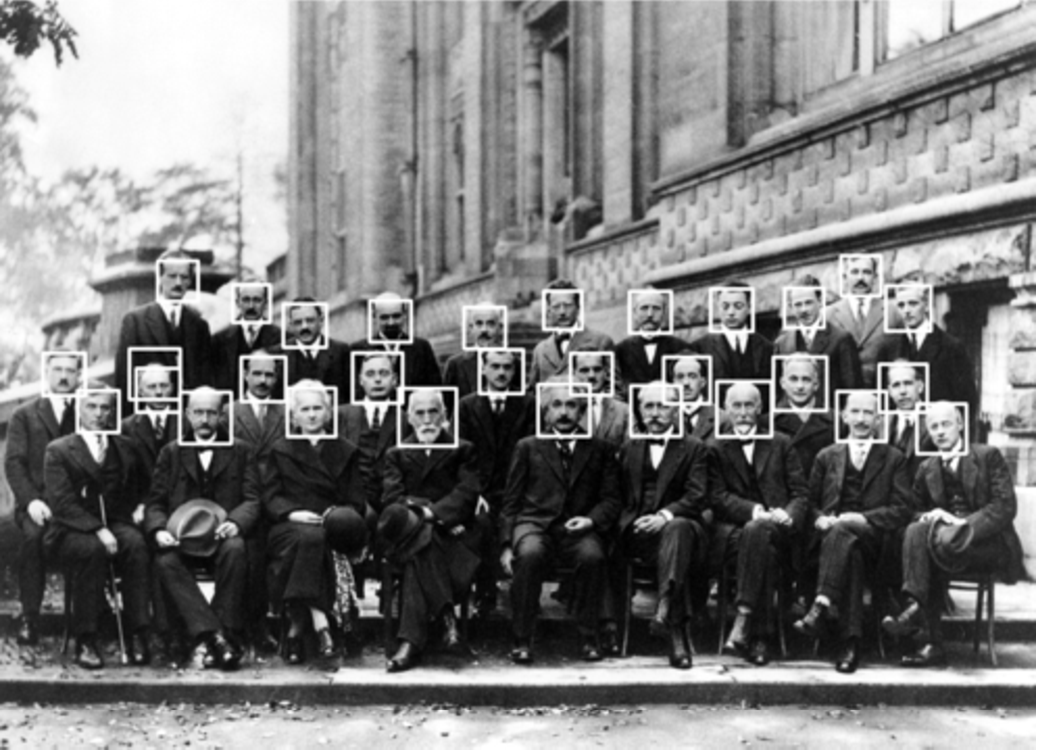
\includegraphics[width=.9\textwidth]{figures/physicist.pdf}
    \label{fig:physicist}
  \end{minipage}%
  \begin{minipage}{0.6\textwidth}
    \centering
    \begin{tabular}{c c c}
      \toprule
      \specialcell{RPi\\Model B}
      & \specialcell{Macbook \\ Model A1502}
      & \specialcell{Workstation\\Xeon E5-1620} \\
      \midrule
      4105 ms & 544 ms & 346 ms \\
      \bottomrule
    \end{tabular}
  \end{minipage}
  \caption{(Left) Face detection with a photograph of the Fifth Solvay
    International Conference on Electrons and Photons. (Right) Processing times
    using Viola-Jones face detector on different machines,with default OpenCV
    parameters.}
  \label{fig:capabilities}
\end{figure}

Our target application environment consists of machines with large range of
computing resources. Earlier, \autoref{sec:swarm-platforms} and
\autoref{tab:embedded} have discussed this dizzying array of machines ranging
from powerful computing units to low-power microcontrollers.  Low-power devices,
such as mobile phones or IoT microcontrollers, are significantly limited in
their processing capabilities. Performing ML inference easily takes seconds to
complete. As shown in \autoref{fig:capabilities}, to detect faces in a photo of
the Fifth Solvay International Conference on Electrons and Photons,\footnote{The
  original image (3000$\times$2171 pixels) is from Wikimedia and in the public
  domain.} it takes more than 4 seconds on a Raspberry Pi (Model B).

One technique is to use the edge and/or the cloud for offloading. While they are
substantially more powerful (7.5$\times$ to 11.9$\times$ in the face detection
task), both the edge and the cloud suffer from variable latency, unstable
connection, and service contention. These issues make it difficult to provide
consistent response times, especially for tail performance. Earlier in
\autoref{fig:edge}, we have shown the characteristics of end devices, the edge,
and the cloud. We then empirically validate the network variation and workload
variation (\autoref{fig:variation}).

\para{Network Variation.} We use the raw data in January 2016 from FCC
\href{https://www.fcc.gov/general/measuring-broadband-america}{Measuring
  Broadband America Program}~\cite{fcc} to validate the large variation in wide
area network. \autoref{fig:fcc-latency} shows the empirical cumulative
distribution function (ECDF) of measured network latency. \textit{Ping} time refers to
the round trip time (RTT) of ICMP echo requests from measurement devices to a
set of target test nodes. \textit{Download} and \textit{Upload} are latency
measured when performing downstream or upstream speed tests. From this figure,
we can see that the latency has 2-3 orders of magnitude difference. The
situation is worse with active traffic. The median network delay increases from
\SI{22}{\ms} to \SI{80}{\ms} under downstream load and \SI{272}{\ms} under
upstream load.

\para{Workload Variation.} \noindent We measure end-to-end latency with
TensorFlow serving~\cite{olston2017tensorflow}, a state-of-the-art serving
system for machine learning models. Specifically, we use
MNIST~\cite{lecun1998mnist} as a case study and study the serving performance
with different level of background load. \autoref{fig:tf-latency} shows the ECDF
with no load, 1K requests per second (RPS) and 5K RPS. From this figure, we can
see that the serving latency has significantly increased when the load
increases. With 1k load, p99.9 latency increases from \SI{3.5}{\ms} to
\SI{22.5}{\ms}. With 5K load, even the median latency increases to
\SI{21.5}{\ms}: a 22.4$\times$ increase from \SI{0.96}{\ms} with no load.

\begin{figure}
  \centering
  \begin{subfigure}[t]{0.4\columnwidth}
    \centering
    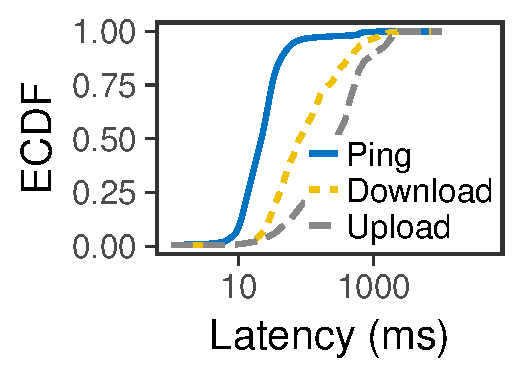
\includegraphics[width=\textwidth]{figures/fcc_latency.pdf}
    \caption{Broadband network latency.}
    \label{fig:fcc-latency}
  \end{subfigure}
  \hspace{2em}
  \begin{subfigure}[t]{0.4\columnwidth}
    \centering
    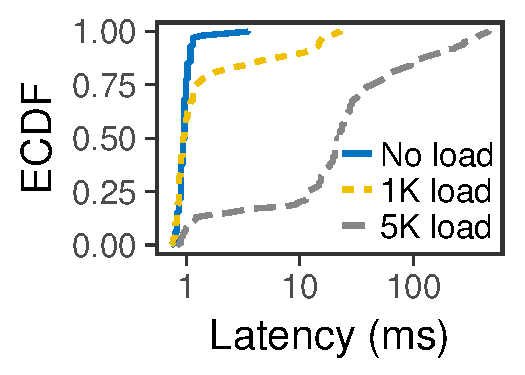
\includegraphics[width=\textwidth]{figures/tf_latency.pdf}
    \caption{TensorFlow serving latency.}
    \label{fig:tf-latency}
  \end{subfigure}
  \caption{(Left) WAN network latency has variation and the latency deteriorates
    during downstream and upstream speed tests. (Right) Server processing
    latency has variation and the latency deteriorates during load increase.}
  \label{fig:variation}
\end{figure}

\subsection{Accuracy-Time Tradeoff}
\label{sec:comp-perf-model}

\begin{figure}[t]
  \centering
  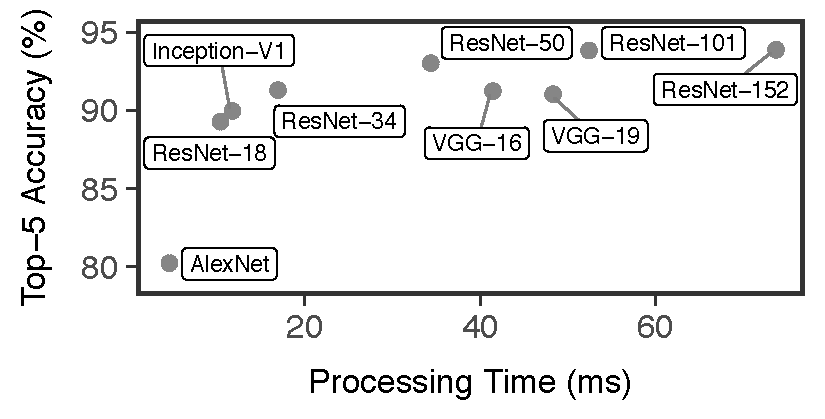
\includegraphics[width=.7\columnwidth]{figures/tradeoff-cnn.pdf}
  \caption{Benchmarks for popular CNN models demonstrate the trade-off between
    application accuracy and processing times. For data source and details,
    refer to
    \href{https://github.com/jcjohnson/cnn-benchmarks}{cnn-benchmarks}~\cite{cnn.benchmarks}.
  }
  \label{fig:cnn-tradeoff}
\end{figure}

Many tasks, especially ML inference, have multiple algorithms, or tunable
parameters for the same algorithm. These options lead to different application
accuracy and processing times. As a result, we can speed up a computation task
by sacrificing accuracy. In this way, many tasks become tractable on end devices
and servers can also tune their computation to accommodate network delays or
address heavy load. Below we show two examples.

\para{Convolutional neural networks (CNN)}. For the past few years, deep
learning and neural networks have gained attention in performing complex machine
learning tasks~\cite{goodfellow2016deep}. Convolutional neural networks (CNNs)
are particularly powerful for computer vision tasks, such as object detection
and image classification. There are many networks available:
AlexNet~\cite{krizhevsky2012imagenet}, Inception~\cite{szegedy2015going},
VGG~\cite{simonyan2014very}, ResNet~\cite{he2016deep}, etc. Huang et al. have
observed the speed/accuracy trade-off and explored this trade-off in an
exhaustive and fair manner~\cite{huang2016speed}. Because this thesis is not
about extensive studies of neural networks, we only summarize one benchmark
result in \autoref{fig:cnn-tradeoff}. The processing times vary from
\SI{4.3}{\ms} to \SI{73.5}{\ms} and the accuracy\footnote{Top-5 accuracy here
  means that the correct label is one of the top 5 predictions made by the
  network.} varies from 80.2\% to 93.8\%.

\para{Viola-Jones Face Detector.} This is an example for one algorithm with
tunable parameters that affect processing times and application
accuracy. Viola-Jones (VJ) cascade face detector~\cite{viola2001rapid}. The
cascade classifier consists of a list of stages, where each stage consists of a
list of weak learners.  The system detects objects in question by moving a
window over the image.  Each stage of the classifier labels the specific region
defined by the current location of the window as either positive or negative –
positive meaning that an object was found or negative means that the specified
object was not found in the image.  Therefore, it has three parameters,

\begin{itemize}[noitemsep, topsep=5pt]
\item \texttt{scale}: how much image size is reduced at each image scale.
\item \texttt{min\_size}: minimum detectable object size.
\item \texttt{min\_neighbors}: how many neighbors each candidate rectangle should
  have to retain it.
\end{itemize}

ML algorithms have many tunable parameters. For many algorithms, processing
times and the accuracy may exhibit \textit{non-linear} behavior with respect to
the parameters. \autoref{fig:vj-tradeoff}.

\begin{figure}[t]
  \centering
  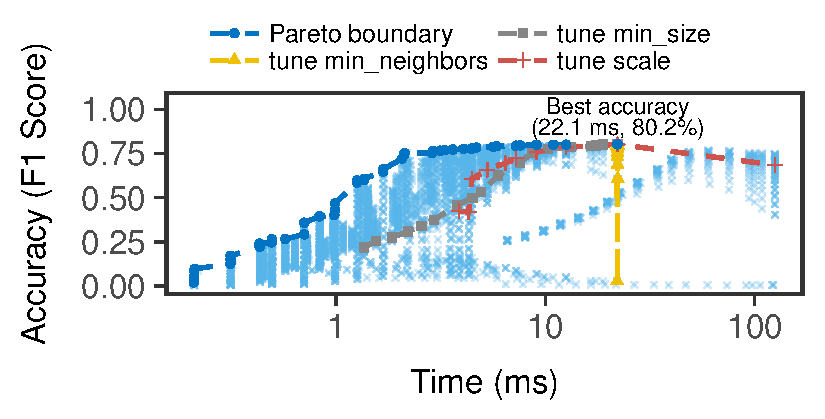
\includegraphics[width=.8\columnwidth]{figures/exhaustive-face.pdf}
  \caption{Complex performance model: spanning multiple dimensions and
    exhibiting non-linear relationship.}
  \label{fig:vj-tradeoff}
\end{figure}

\subsection{Performance Modeling Challenges}
\label{sec:challenges}

The two strawman solutions for predicting a near optimal cloud configuration are
modeling and searching.

\para{Exhaustive Search for Accurate Modeling is Too Expensive.} One way to
model performance and then pick the best configuration based on this
model.~\autoref{fig:vj-tradeoff}. However, this methodology has poor
adaptivity. Building a model that works for a variety of applications and cloud
configura- tions can be difficult because the knowledge of the inter- nal
structure of specific applications is needed to make the model
effective. Moreover, building a model through human intervention for every new
application can be tedious. Static searching for the best cloud
configuration. An other way is to exhaustively search for the best cloud
configuration without relying on an accurate perfor- mance model. However, this
methodology has high over- head. With 40 instance types at Amazon EC2 and tens
of cluster sizes for an application, if not careful, one could end up needing
tens if not hundreds of runs to identify the best instance. In addition, tryinpg
each cloud con- figuration multiple times to get around the dynamics in the
cloud (due to resource multiplexing and stragglers) would exacerbate the problem
even further.

To reduce the search time and cost, one could use co- ordinate descent and
search one dimension at a time. Co- ordinate descent could start with searching
for the opti- mal CPU/RAM ratio, then the CPU count per machine, then cluster
size, and finally disk type. For each dimen- sion, we could fix the other
dimensions and search for the cheapest configuration possible. This could lead
to suboptimal decisions if for example, because of bad ap- plication
configuration a dimension is not fully explored or there are local minima in the
problem space.

%%% Local Variables:
%%% mode: latex
%%% TeX-master: "../compute"
%%% End:
